\documentclass{article}

% packages
\usepackage{amsmath, amsthm, thmtools, amsfonts, amssymb, luacode, catchfile, tikzducks, hyperref, ifthen}
\ifcsname c@kobocompile\endcsname
	\usepackage[a5paper, total={1072pt, 1448pt}, margin=10pt, includeheadfoot]{geometry} % set page margins
\else
	\usepackage[a4paper, margin=50pt, includeheadfoot]{geometry}
\fi
\usepackage[shortlabels]{enumitem}
\usepackage[skip=3pt, indent=0pt]{parskip}

% language
\usepackage[bidi=basic, layout=tabular, provide=*]{babel}
\ifcsname c@english\endcsname
	\babelprovide[main, import]{english}
\else
	\babelprovide[main, import]{hebrew}
	\babelprovide{rl}
\fi
%\babelfont{rm}{Libertinus Serif}
\babelfont{rm}[Renderer=Harfbuzz]{Libertinus Serif}
\babelfont{sf}{Libertinus Sans}
\babelfont{tt}{Libertinus Mono}

% style
\AddToHook{cmd/section/before}{\clearpage}	% Add line break before section
\linespread{1.3}
\setcounter{secnumdepth}{0}		% Remove default number tags from sections, this won't do well with theorems
\AtBeginDocument{\setlength{\belowdisplayskip}{3pt}}
\AtBeginDocument{\setlength{\abovedisplayskip}{3pt}}
\graphicspath{ {../images/} }

% operators
\DeclareMathOperator\cis{cis}
\DeclareMathOperator\Sp{Sp}
\DeclareMathOperator\tr{tr}
\DeclareMathOperator\im{Im}
\DeclareMathOperator\re{Re}
\DeclareMathOperator\diag{diag}
\DeclareMathOperator*\lowlim{\underline{lim}}
\DeclareMathOperator*\uplim{\overline{lim}}
\DeclareMathOperator\rng{rng}
\DeclareMathOperator\Sym{Sym}
\DeclareMathOperator\Arg{Arg}
\DeclareMathOperator\Log{Log}
\DeclareMathOperator\dom{dom}
\DeclareMathOperator\supp{Supp}
\DeclareMathOperator\var{Var}
\DeclareMathOperator\cov{Cov}

% commands
%\renewcommand\qedsymbol{\textbf{מש''ל}}
%\renewcommand\qedsymbol{\fbox{\emoji{lizard}}}
\newcommand{\Aa}[0]{\mathcal{A}}
\newcommand{\Bb}[0]{\mathcal{B}}
\newcommand{\CC}[0]{\mathbb{C}}
\newcommand{\Cc}[0]{\mathcal{C}}
\newcommand{\EE}[0]{\mathbb{E}}
\newcommand{\FF}[0]{\mathbb{F}}
\newcommand{\Ff}[0]{\mathcal{F}}
\newcommand{\Ii}[0]{\mathcal{I}}
\newcommand{\Gg}[0]{\mathcal{G}}
\newcommand{\Ll}[0]{\mathcal{L}}
\newcommand{\Mm}[0]{\mathcal{M}}
\newcommand{\NN}[0]{\mathbb{N}}
\newcommand{\Nn}[0]{\mathcal{N}}
\newcommand{\PP}[0]{\mathbb{P}}
\newcommand{\Pp}[0]{\mathcal{P}}
\newcommand{\QQ}[0]{\mathbb{Q}}
\newcommand{\RR}[0]{\mathbb{R}}
\newcommand{\Rr}[0]{\mathcal{R}}
\newcommand{\Ss}[0]{\mathcal{S}}
\newcommand{\TT}[0]{\mathbb{T}}
\newcommand{\Uu}[0]{\mathcal{U}}
\newcommand{\Vv}[0]{\mathcal{V}}
\newcommand{\Ww}[0]{\mathcal{W}}
\newcommand{\ZZ}[0]{\mathbb{Z}}
\newcommand{\acts}[0]{\circlearrowright}
\newcommand{\explain}[2] {
	\begin{flalign*}
		 && \text{#2} && \text{#1}
	\end{flalign*}
}
\newcommand{\maketitleprint}[0]{ \begin{center}
	%\begin{tikzpicture}[scale=3]
	%	\duck[graduate=gray!20!black, tassel=red!70!black]
	%\end{tikzpicture}	
	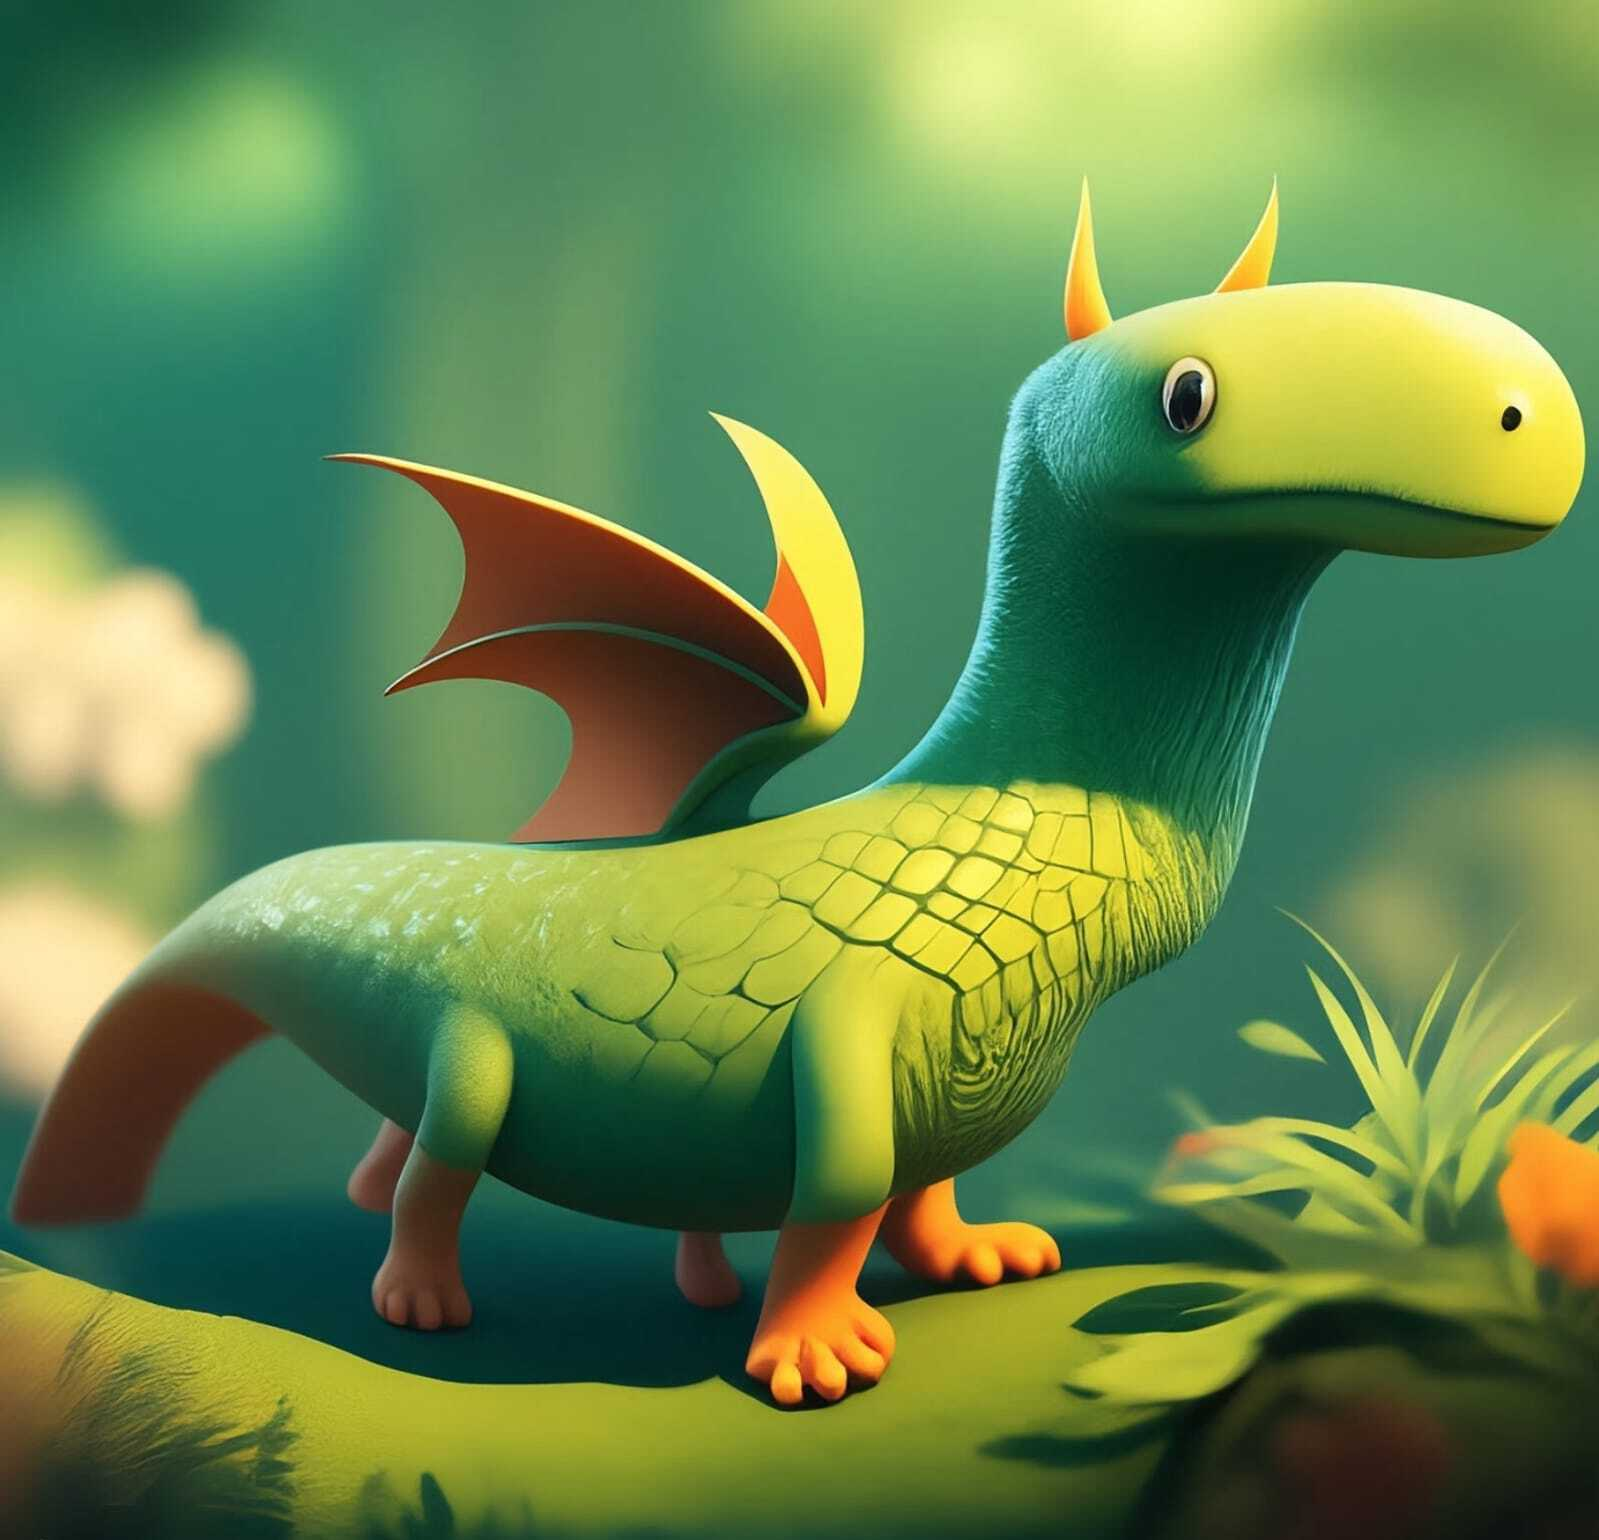
\includegraphics[width=6cm]{cover}
\end{center}
}

% theorem commands
\newtheoremstyle{c_remark}
	{}	% Space above
	{}	% Space below
	{}% Body font
	{}	% Indent amount
	{\bfseries}	% Theorem head font
	{}	% Punctuation after theorem head
	{.5em}	% Space after theorem head
	{\thmname{#1}\thmnumber{ #2}\thmnote{ \normalfont{\text{(#3)}}}}	% head content
\newtheoremstyle{c_definition}
	{3pt}	% Space above
	{3pt}	% Space below
	{}% Body font
	{}	% Indent amount
	{\bfseries}	% Theorem head font
	{}	% Punctuation after theorem head
	{.5em}	% Space after theorem head
	{\thmname{#1}\thmnumber{ #2}\thmnote{ \normalfont{\text{(#3)}}}}	% head content
\newtheoremstyle{c_plain}
	{3pt}	% Space above
	{3pt}	% Space below
	{\itshape}% Body font
	{}	% Indent amount
	{\bfseries}	% Theorem head font
	{}	% Punctuation after theorem head
	{.5em}	% Space after theorem head
	{\thmname{#1}\thmnumber{ #2}\thmnote{ \text{(#3)}}}	% head content

\ifcsname c@english\endcsname
	\theoremstyle{plain}
	\newtheorem{theorem}{Theorem}[section]
	\newtheorem{lemma}[theorem]{Lemma}
	\newtheorem{proposition}[theorem]{Proposition}
	\newtheorem*{proposition*}{Proposition}
	%\newtheorem{corollary}[theorem]{אין חלופה עברית}

	\theoremstyle{definition}
	\newtheorem{definition}[theorem]{Definition}
	\newtheorem*{definition*}{Definition}
	\newtheorem{example}{Example}[section]
	\newtheorem{exercise}{Exercise}[section]

	\theoremstyle{remark}
	\newtheorem*{remark}{Remark}
	\newtheorem*{solution}{Solution}
	\newtheorem{conclusion}[theorem]{Conclusion}
	\newtheorem{notation}[theorem]{Notation}
\else
	\theoremstyle{c_plain}
	\newtheorem{theorem}{משפט}[section]
	\newtheorem{lemma}[theorem]{למה}
	\newtheorem{proposition}[theorem]{טענה}
	\newtheorem*{proposition*}{טענה}
	%\newtheorem{corollary}[theorem]{אין חלופה עברית}

	\theoremstyle{c_definition}
	\newtheorem{definition}[theorem]{הגדרה}
	\newtheorem*{definition*}{הגדרה}
	\newtheorem{example}{דוגמה}[section]
	\newtheorem{exercise}{תרגיל}[section]

	\theoremstyle{c_remark}
	\newtheorem*{remark}{הערה}
	\newtheorem*{solution}{פתרון}
	\newtheorem{conclusion}[theorem]{מסקנה}
	\newtheorem{notation}[theorem]{סימון}
\fi

% Questions related commands
\newcounter{question}
\setcounter{question}{1}
\newcounter{sub_question}
\setcounter{sub_question}{1}

\ifcsname c@english\endcsname
	\newcommand{\question}[1][0]{
		\ifthenelse{#1 = 0}{}{\setcounter{question}{#1}}
		\section{Question \arabic{question}}
		\addtocounter{question}{1}
		\setcounter{sub_question}{1}
	}

	\newcommand{\subquestion}[1][0]{
		\ifthenelse{#1 = 0}{}{\setcounter{sub_question}{#1}}
		\subsection{Part \alph{sub_question}}
		\addtocounter{sub_question}{1}
	}
\else
	\newcommand{\question}[1][0]{
		\ifthenelse{#1 = 0}{}{\setcounter{question}{#1}}
		\section{שאלה \arabic{question}}
		\addtocounter{question}{1}
		\setcounter{sub_question}{1}
	}

	\newcommand{\subquestion}[1][0]{
		\ifthenelse{#1 = 0}{}{\setcounter{sub_question}{#1}}
		\subsection{סעיף \localecounter{letters.gershayim}{sub_question}}
		\addtocounter{sub_question}{1}
	}
\fi

% import lua and start of document
\directlua{common = require ('../common')}

\GetEnv{AUTHOR}

% headers
\author{\AUTHOR}
\date\today

\title{פתרון מטלה 05 --- פונקציות מרוכבות, 80519}

\begin{document}
\maketitle
\maketitleprint{}

\question{}
נתאר את צורתן של המסילות הבאות במישור המרוכב ונחשב את אורכן.

\subquestion{}
$\gamma(t) = i \sin(t^2)$ עבור $t \in [-\sqrt{\frac{\pi}{2}}, \sqrt{\frac{\pi}{2}}]$.
\begin{solution}
	צורתה הקו $[0, i]$, הכיוון שלה הוא תחילה לראשית הצירים ואז ל־$(0, i)$.
	נוכל כבר להסיק שאורכה הוא בדיוק $2$, אך נחשב גם על־ידי ההגדרה:
	\[
		L(\gamma)
		= \int_{-\sqrt{\frac{\pi}{2}}}^{\sqrt{\frac{\pi}{2}}} |\gamma'(t)|\ dt
		= \int_{-\sqrt{\frac{\pi}{2}}}^{\sqrt{\frac{\pi}{2}}} \cos(t^2) \cdot 2t\ dt
		= |\sin(t^2)|_{-\sqrt{\frac{\pi}{2}}}^{\sqrt{\frac{\pi}{2}}}
		= 1 + 1
	\]
\end{solution}

\subquestion{}
$\gamma(t) = e^{it}$ עבור $t \in [0, 7\pi]$.
\begin{solution}
	אנו יודעים מתרגולי עבר כי מסילה זו היא מעגל יחידה (שלוש וחצי פעמים) וכן כיוונה נגד כיוון השעון.
	גם הפעם אנו כבר יודעים שמתקיים $L(\gamma) = 2\pi \cdot \frac{7}{2}$, אך נחשב בכל זאת:
	\[
		L(\gamma)
		= \int_0^{7\pi} |\gamma'(t)|\ dt
		= \int_0^{7\pi} |i e^{it}|\ dt
		= \int_0^{7\pi} \sqrt{\cos^2 t + \sin^2 t}\ dt
		= \int_0^{7\pi} 1\ dt
	\]
\end{solution}

\subquestion{}
$\gamma(t) = t e^{\frac{\pi i}{4}}$ עבור $t \in [0, 10]$.
\begin{solution}
	נבחין כי $e^{\frac{\pi i}{4}}$ הוא ערך קבוע ומשמעותו שלעקומה תהיה זווית של $\frac{\pi}{4}$ מראשית הצירים. עוד אנו יודעים כי יש מכפלה ב־$t$ ולכן זה ישר שאורכו 10, מתחיל בראשית וזז החוצה ממנה בזווית זו מציר ה־$x$.
	גם הפעם אנו יודעים את האורך אך נחשב
	\[
		\int_0^{10} |\gamma'(t)|\ dt
		= \int_0^{10} |e^{\frac{\pi i}{4}}|\ dt
		= \int_0^{10} 1\ dt
	\]
\end{solution}

\subquestion{}
$\gamma(t) = t e^{it}$ עבור $t \in [0, 4\pi]$.
\begin{solution}
	מהסעיפים הקודמים נסיק כי זהו ישר מהראשית שעובר סיבוב ככל שהוא מתרחק ממנה, דהינו זוהי ספירלה נגד כיוון השעון שמתחילה ב־$0$ ומסתיימת בנקודה $4\pi + i0$.
	לבסוף נבחין גם שהספירלה מבצעת שני סיבובים שלמים בתחום הגדרתה. \\*
	הפעם אין לנו דרך גאומטרית לחשב את השטח ונחשב על־ידי ההגדרה בלבד:
	\[
		\int_{0}^{4\pi} |\gamma'(t)|\ dt
		= \int_{0}^{4\pi} |e^{it} (1 + it)|\ dt
		= \int_0^{4\pi} \sqrt{1 + t^2}\ dt
	\]
	בהצבה $t = \sinh(\theta)$ נקבל
	\begin{align*}
		\int_0^{4\pi} \sqrt{1 + t^2}\ dt
		& = \int_0^{\sinh^{-1}(4\pi)} \sqrt{1 + \sinh^2(\theta)} \cosh(\theta)\ d\theta \\
		& = \int_0^{\sinh^{-1}(4\pi)} \cosh(\theta) \cosh(\theta)\ d\theta \\
		& = \int_0^{\sinh^{-1}(4\pi)} \cosh^2(\theta)\ d\theta \\
		& = \frac{1}{2} \int_0^{\sinh^{-1}(4\pi)} \cosh(2\theta) + 1\ d\theta \\
		& = \frac{1}{2} \sinh^{-1}(4\pi) + \frac{1}{4} \sinh(2 \sinh^{-1}(\theta)) \\
		& = \frac{1}{2} \sinh^{-1}(4\pi) + 4 \pi^2
	\end{align*}
\end{solution}

\question{}
נמצא פרמטריזציה לעקומות הסגורות הבאות ונחשב את אורכן.

\subquestion{}
משולש פיצה ברדיוס $r$ המתחיל בראשית, ממשיך על הכיוון החיובי של ציר ה־$x$ ויש לו זווית $\theta \in (0, \frac{\pi}{2})$.
\begin{solution}
	נתחיל ב־$\gamma_1(t) = t$ עבור $t \in [0, 1]$, ובאותו אופן גם $\gamma_3 = e^{\theta i} t$ לאותו תחום. \\*
	באופן דומה גם $\gamma_2(t) = e^{it}$ עבור $t \in [0, \theta]$, ונגדיר $\gamma = \gamma_1 + \gamma_2 + \gamma_3$ בהתאם להגדרה בהרצאה. \\*
	האורך בהתאם לשאלה 1 הוא $2 + \theta$.
\end{solution}

\subquestion{}
מלבן בגודל $a \times b$ המתחיל בראשית וממשיך על החלק השלילי של הציר הממשי.
\begin{solution}
	נגדיר $\gamma_1(t) = -t$ עבור $t \in [0, a]$, ובהתאם $\gamma_2(t) = -a + ti$ עבור $t \in [0, b]$. \\*
	נגדיר גם $\gamma_3(t) = t(-a + bi) + (1 - t)(bi)$ עבור $t \in [0, 1]$ ולבסוף $\gamma_4(t) = (1 - t) bi$ עבור $t \in [0, 1]$. \\*
	נגדיר את הסכום כבסעיף הקודם $\gamma$ ומשאלה 1 נובע $L(\gamma) = 2a + 2b$.
\end{solution}

\subquestion{}
משולש המתחיל בראשית ויוצר משולש ישר זווית ושווה שוקיים עם צלע בסיס באורך 2 המונחת על החלק החיובי של הציר המדומה.
\begin{solution}
	נגדיר $\gamma_1(t) = 0(1 - t) + (t)(2 + i \frac{\sqrt{2}}{2})$ עבור $t \in [0, 1]$. \\*
	נגדיר גם $\gamma_2(t) = (1  - t)(2 + i \frac{\sqrt{2}}{2}) + t (0 + 2i)$ עבור תחום זהה, \\*
	ולבסוף נגדיר $\gamma_3(t) = (1 - t) (0 + 2i)$ עבור תחום זהה. \\*
	נגדיר $\gamma = \gamma_1 + \gamma_2 + \gamma_3$ וכן $L(\gamma) = 2 + 2 \sqrt{2}$.
\end{solution}

\subquestion{}
שני מעגלים ברדיוס 1 המשיקים בראשית עם מרכזים על הציר המדומה.
\begin{solution}
	התרגיל לא ברור, אני מנחש ש־$\gamma(t) = e^{it} + i$ עבור $t \in [0, 4\pi]$ שכן אלה הם שני מעגלים שעוברים בראשית הצירים ומשיקים שם, וכמובן $L(\gamma) = 4\pi$.
\end{solution}

\question{}
נגדיר את התחום
\[
	A = \{z \in \CC \mid 0 \le \re(z) \le \im(z), 1 \le \im(z) \le 2\}
\]
נתאר את התחום ונחשב את השטח של $\Log(A)$.
\begin{solution}
	על־ידי בדיקת התנאים נסיק שמדובר בטרפז שקודקודיו הם $(0, 1), (1, 1), (2, 2), (0, 2)$. \\*
	לכן גם נוכל להסיק ישירות ששטחו הוא $\frac{(1 + 2) \cdot 1}{2} = \frac{3}{2}$. \\*
	נעבור לחישוב השטח של $\Log(A)$ בתחום, כמובן הפונקציה מוגדרת בתחום ולכן יש לנו הצדקה לדבר על שטחה שם, נחשב את השטח בדומה לאופן בו הוא חושב בתרגול.
	\begin{align*}
		\iint_{\Log(A)} 1\ d|w|
		& = \iint_A {|\Log'(z)|}^2\ d|z| \\
		& = \iint_A \frac{1}{z \overline{z}}\ dz \\
		& = \iint_A \frac{1}{x^2 + y^2}\ dx\ dy \\
		& = \int_1^2 \left(\int_0^y \frac{1}{x^2 + y^2}\ dx\right)\ dy \\
		& = \int_1^2 \frac{1}{y} \arctan(\frac{y}{y}) - 0\ dy \\
		& = \frac{\pi}{4} \cdot (\log(2) - \log(1))
	\end{align*}
\end{solution}

\question{}
נגדיר $\gamma_0 : [0, 3] \to \CC$ על־ידי
\[
	\gamma_0(t) = \begin{cases}
		t & t \in [0, 1] \\
		1 + e^{-\frac{\pi i}{3}} (t - 1) & t \in [1, 2] \\
		1 + e^{-\frac{\pi i}{3}} + e^{\frac{\pi i}{3}} (t - 2) & t \in [1, 2] \\
	\end{cases}
\]
משלוש שווה־צלעות, ונגדיר באופן אינדוקטיבי מסילה $\gamma_n$ להיות המסילה $\gamma_{n - 1}$ כאשר מחליפים כל קטע ישר בה בעותק מוקטן ומסובב של המסילה
\[
	\alpha(t) = \begin{cases}
		\frac{4}{3} t & t \in [0, \frac{1}{4}] \\
		\frac{1}{3} + \frac{4}{3} e^{\frac{\pi i}{3}} (t - \frac{1}{4}) & t \in [\frac{1}{4}, \frac{1}{2}] \\
		\frac{1}{3} + \frac{1}{3} e^{\frac{\pi i}{3}} + \frac{4}{3} e^{-\frac{\pi i}{3}} (t - \frac{1}{2}) & t \in [\frac{1}{2}, \frac{3}{4}] \\
		\frac{2}{3} + \frac{4}{3} (t - \frac{3}{4}) & t \in [\frac{3}{4}, 1]
	\end{cases}
\]

\subquestion{}
נוכיח ש־$(\gamma_n)$ מתכנסת במידה שווה למסילה $\gamma$ כלשהי.
\begin{proof}
	נבחן את ההפרשים של המסילות, קרי $\gamma_n - \gamma_{n - 1}$, ונבחין כי הפרש זה הוא תוספת המשולשים החדשים שנוצרו מכל קו שהיה קודם לכן,
	ונוכל להוכיח ישירות מהגדרת $\alpha$ שמתקיים $\max \im \alpha = \frac{1}{3}$. \\*
	עוד נבחין שיש ב־$\gamma_n$ בדיוק $3 \cdot 4^n$ קטעים $C^1$ (קטעים ישרים), וכן שאורכם זהה והוא $\frac{1}{3^n}$. כל זאת ניתן להוכיח באינדוקציה על הגדרת המסילות. \\*
	אם כך $\max |\gamma_n(t) - \gamma_{n - 1}(t)| = \frac{1}{3} \cdot \frac{1}{3^n}$ ולכן ממבחן $M$ של ויירשטראס טור ההפרשים מתכנס במידה שווה, כלומר $\gamma_n \to \gamma$ במידה שווה.
\end{proof}

\subquestion{}
נוכיח כי $L(\gamma_n) \xrightarrow[n \to \infty]{} = \infty$.
\begin{proof}
	למעשה מצאנו שמתקיים $L(\gamma_n) = 3 \cdot 4^n \cdot \frac{1}{3^n} = 3 \cdot {\left(\frac{4}{3}\right)}^n$, וזוהי כמובן סדרה מתבדרת ל־$\infty$.
\end{proof}

\subquestion{}
נסמן ב־$A_n$ את השטח הכלוא ב־$\gamma_n$, ונחשב את $\lim_{n \to \infty} A_n$.
\begin{solution}
	באופן דומה לסעיף א', נבחין שב־$\gamma_n - \gamma_{n - 1}$ ישנם שלושה משולשים חדשים, שטח כל אחד הוא $\frac{1}{2} \sin(\frac{\pi}{3}) \frac{1}{3^n} \cdot \frac{1}{3^n}$ לפי חישוב ישיר, ולכן
	\[
		A_n = \frac{1}{2} \sin(\frac{\pi}{3}) + \sum_{i = 1}^{n} \sin(\frac{\pi}{3}) \frac{3 (4^n - 4^{n - 1})}{4 \cdot 9^n}
		= \frac{1}{2} \sin(\frac{\pi}{3}) (1 + \frac{1}{2} \sum_{i = 1}^{n} \frac{4^{n - 1} }{\cdot 9^{n - 1}})
	\]
	על־ידי חישוב כמות המשולשים שנוספים לפי מספר הקווים שמתווספים, כל שני קווים מרכיבים משולש אחד.
	ולבסוף נקבל
	\[
		\lim_{n \to \infty} A_n
		= \frac{1}{2} \sin(\frac{\pi}{3}) (1 + \frac{1}{2} \cdot \frac{1}{1 - \frac{4}{9}})
		= \sin(\frac{\pi}{3}) \frac{19}{20}
	\]
\end{solution}

\end{document}
